\begin{comment}
\section{CPS Security Challenges}
\begin{figure*}
\centering
\includegraphics[width=0.95\textwidth]{CPS-Survey (4)/images/cps-security-challenges.png}
\caption{Overview of CPS Security Challenges and Classification}
\label{fig:overview}
\end{figure*}
Cyber-Physical Systems (CPS) face a wide range of security challenges due to their combination of digital and physical components. These systems, which are used in areas like healthcare, transportation, and critical infrastructure, must handle threats from both cyber and physical domains. The complexity of these systems makes them difficult to protect. To better understand these security issues, we can group them into four themes: system-level vulnerabilities, threats and attack types, security measures and responses, and external factors such as regulations, privacy concerns, and the human element.

\subsection{System-Level Vulnerabilities and Constraints}

CPS often have significant limitations that affect their security. One of the main challenges is the resource constraints that many devices in a CPS system face. These devices, such as sensors and actuators, usually have limited computational power, memory, and energy. This makes it difficult to apply traditional security techniques like complex encryption or advanced intrusion detection systems. Since many CPS are designed for long-term use and operate continuously, they cannot afford to stop or slow down for security updates. For example, in healthcare or industrial control systems, CPS must work in real time. This means that any security feature that adds delays could interfere with critical operations and potentially cause harm \cite{30,34,36}.

Another issue is the cross-domain complexity of CPS. These systems integrate both physical components (such as machines, robots, and sensors) with cyber components (like networks and software). This integration creates new challenges because attacks can target either the cyber or physical aspects of the system. An attacker might try to disrupt the software or attack physical parts of the system, such as tampering with a sensor, which could cause the system to malfunction. Unlike traditional IT systems, the consequences of an attack in CPS are not limited to data breaches—they can lead to physical damage or even threats to human safety \cite{31,34}.

The problem is worsened by the fact that many CPS rely on legacy systems. These older systems were not designed with modern cybersecurity threats in mind. Upgrading them is often complicated or even impossible without interrupting their operations. Many of these systems were built to last for decades, so they still use outdated protocols and hardware that can be easily exploited by attackers. Applying security patches to these systems is not always possible, especially when updating them might require long downtimes, which are unacceptable for critical operations like power grids or healthcare equipment \cite{40,42}.

Another important challenge in securing CPS is scalability. As CPS expand into larger networks, such as smart cities or large industrial plants, it becomes harder to secure all the devices in the system. A typical CPS can include thousands of sensors, actuators, and controllers, all connected through networks. Managing security across such a large number of devices without slowing down operations is a major challenge. As the system grows, the security solution must also be able to scale up to handle the increased complexity without causing delays or failures \cite{36,38}.

Finally, CPS systems are often interconnected, which introduces the risk of cascading effects. If one part of the system is attacked, it can affect other parts of the system. For example, if a hacker attacks a single component in a power grid, it could cause a blackout that affects an entire city. This interconnectedness means that even a small attack can have widespread consequences, making it crucial to protect every part of the system equally well \cite{37,41}.

\subsection{Threats and Attack Vectors}

CPS faces a wide variety of threats, including both traditional cyber-attacks and physical attacks. One of the main challenges in securing CPS is the threat diversity. CPS can be attacked through both digital means, like malware, denial of service (DoS) attacks, or hacking, and physical means, like tampering with devices or sabotaging equipment. For example, attackers can hack into the control systems of a CPS and manipulate sensor data, causing the system to make wrong decisions. They could also physically tamper with a sensor to feed incorrect information into the system, leading to malfunctions. These attacks can cause both digital and physical harm, which makes securing CPS more difficult than traditional IT systems \cite{30,34,40}.

In addition to the variety of attacks, CPS also faces advanced threats that are harder to detect and defend against. These threats include sophisticated attacks like zero-day vulnerabilities, which exploit unknown weaknesses in the system before they can be patched. Attackers can also coordinate multiple attacks at once, targeting different parts of the system to cause widespread damage. These advanced threats often avoid triggering traditional security alarms, making them particularly dangerous in CPS environments where the consequences of a successful attack can be severe, such as equipment failure or threats to human safety \cite{34,36,37}.

Another important issue in CPS security is the threat posed by insider threats. Unlike external hackers, insiders already have authorized access to the system, which makes their actions harder to detect. These threats can come from disgruntled employees, contractors, or anyone who has access to the system. Insider threats can also be unintentional, such as when an employee accidentally introduces vulnerabilities by misconfiguring a device or using weak security practices. Protecting against insider threats requires strong access control, monitoring, and proper training to ensure that employees do not accidentally or intentionally harm the system \cite{35,39}.

\subsection{Security Measures and Responses}

Securing CPS requires unique security measures and strategies. One of the main challenges in protecting CPS is the need for fast and accurate detection and response systems. Traditional security tools, such as firewalls and network-based intrusion detection systems, are not enough for CPS environments. In CPS, attacks can affect both digital and physical parts of the system, so security systems must monitor for unusual behavior in the physical components, like sensors or actuators, as well as the cyber components. This means that new kinds of detection methods are needed, which can recognize when something is wrong not just in the network traffic, but also in the physical operation of the system \cite{30,33}.

Another key aspect of CPS security is physical threats. CPS must be designed to continue operating even during an attack. These systems need to be able to detect a problem quickly, isolate the affected part of the system, and continue working without causing harm. For example, in a smart grid, if one part of the system fails due to a cyber-attack, the other parts of the grid should continue working to prevent a large-scale blackout. Building resilience into CPS is critical because these systems often control essential services, and any downtime could have serious consequences \cite{33,41}.

However, one of the biggest challenges in CPS security is the efficiency tradeoff. Implementing strong security features, such as encryption or multi-factor authentication, can slow down the system. This is a problem in CPS environments that require real-time responses, like autonomous vehicles or emergency systems. In these cases, even a small delay caused by security processes can have dangerous consequences. For example, if an autonomous vehicle takes too long to process data because of a security check, it could fail to avoid an accident. Therefore, CPS security solutions must be lightweight and efficient, providing protection without introducing significant delays \cite{30,31,33}.

\subsection{Regulatory, Privacy, and Human Factors}

In addition to technical challenges, CPS security is also influenced by external factors like government regulations, privacy concerns, and human involvement. One major issue is the lack of standardized regulations. While some industries, like the electric power sector, have developed cybersecurity standards (such as the North American Electric Reliability Corporation (NERC) standards), many other CPS sectors do not have clear and enforceable security policies. Without standardized regulations, different CPS systems may be held to different levels of security, leaving some critical systems vulnerable to attack. Moreover, many regulations are outdated and have not kept pace with new technological developments, meaning that they may not fully address modern threats \cite{30,32,42}.

Another critical concern in CPS is data integrity and privacy. CPS collect vast amounts of data, including sensitive personal information in applications like healthcare or smart cities. Ensuring that this data is protected from unauthorized access and tampering is crucial. If an attacker gains access to control data or sensor readings, they could alter the system's behavior and cause real-world harm. At the same time, CPS must also ensure the privacy of users, especially in systems that handle personal information, such as medical devices or smart home systems. Protecting privacy while maintaining system functionality is a delicate balance that designers must carefully manage \cite{31,36,38}.

Finally, there are significant educational gaps in CPS security. Many engineers, operators, and employees who manage CPS systems are not trained in the specific security threats that CPS face. Without specialized training and awareness, even simple security problems can go undetected, increasing the risk of attacks. Many organizations do not prioritize security training for their staff, which leads to a false sense of security. Addressing these educational gaps is critical to improving the overall security posture of CPS, as well-trained personnel can help prevent attacks and ensure that systems are properly protected \cite{39,43}.
    
\end{comment}

\begin{comment}
    
\section{CPS Security Challenges}
\begin{figure*}
\centering
\includegraphics[width=0.95\textwidth]{/images/cps-security-challenges.png}
\caption{Overview of CPS Security Challenges and Their Classifications}
\label{fig:overview}
\end{figure*}

Cyber-Physical Systems (CPS) are inherently complex due to their combination of digital and physical components, which interact in real-time environments across sectors such as healthcare, transportation, and critical infrastructure. This convergence exposes CPS to a unique blend of vulnerabilities and challenges, which we can broadly group into four categories: system-level vulnerabilities, threats and attack vectors, security measures and responses, and external factors like regulations, privacy, and human involvement. This section provides an integrated analysis of these challenges and explores possible solutions.

\subsection{System-Level Vulnerabilities and Constraints}

CPS face significant system-level vulnerabilities that stem from the resource limitations of their components, the cross-domain complexity of their architecture, and the continued use of legacy systems. Devices in CPS environments, such as sensors and actuators, often have constrained computational power, memory, and energy resources, making it difficult to implement standard security mechanisms like encryption and intrusion detection \cite{30,34,36}. These constraints are further compounded by the need for CPS to operate continuously without downtime, particularly in sectors where real-time operation is critical, such as healthcare and industrial control systems \cite{31,36}. As a result, these systems cannot afford delays due to complex security updates or processes. To tackle these limitations, lightweight security solutions such as elliptic curve cryptography (ECC) and efficient anomaly detection techniques are increasingly adopted to balance the need for security with performance demands \cite{30,34}.

The cross-domain nature of CPS adds another layer of complexity to their security. Unlike traditional IT systems, CPS integrate both physical components—such as machines, robots, and sensors—with cyber elements, including networks and software. This tight coupling of the physical and cyber domains creates vulnerabilities that can be exploited by attackers in multiple ways \cite{31,34}. Attacks on CPS can target either the digital or the physical components; for instance, cyberattacks can manipulate sensor readings, while physical attacks can directly affect actuators or other hardware. Such attacks can lead to not only data breaches but also physical damage or significant threats to human safety \cite{30,34,40}.

Legacy systems pose additional challenges. Many CPS environments, particularly in critical infrastructure like power generation and healthcare, rely on legacy hardware and outdated protocols that were not designed with modern cybersecurity threats in mind \cite{40,42}. Updating or replacing these systems is often cost-prohibitive and operationally risky, leading to continued reliance on technology that lacks essential security capabilities. To mitigate the risks associated with these legacy systems, practices such as network segmentation and virtual patching are often used to create temporary security barriers \cite{40,42}.

The interconnectedness and scale of CPS also lead to challenges related to scalability and cascading effects. In large-scale CPS networks—such as smart cities or extensive industrial operations—thousands of devices are interconnected, increasing the attack surface. If a single vulnerable component is compromised, it can trigger cascading failures that affect the entire system \cite{36,38}. For instance, a compromised sensor in a power grid could lead to widespread blackouts, as was observed in the 2003 Northeast blackout, where a failure in a single monitoring tool had far-reaching consequences. Hierarchical security management, where local control points are established to manage smaller segments of the network, is one approach that can help mitigate these risks by isolating failures and reducing overall system vulnerability \cite{37,41}.

\subsection{Threats and Attack Vectors}

CPS are exposed to a broad spectrum of threats, from traditional cyberattacks to physical sabotage, due to the diverse ways in which these systems operate and interact. One of the critical security challenges lies in the range and diversity of potential attack vectors. Digital attacks, such as malware, denial of service (DoS) attacks, and advanced persistent threats (APTs), can manipulate data or disrupt system operations \cite{30,34,40}. Meanwhile, physical threats—such as tampering with sensors or other hardware—can compromise the integrity of the physical components of the system \cite{30,34}. This dual nature of threats makes CPS security inherently more complex compared to traditional IT systems.

Advanced threats, such as zero-day vulnerabilities, present a particularly serious risk to CPS because these vulnerabilities are often unknown to developers and security professionals, allowing attackers to exploit them before they are patched \cite{34,36,37}. Moreover, attackers are increasingly leveraging AI to identify vulnerabilities or automate coordinated attacks, further complicating defense mechanisms. Such attacks are difficult to detect because they may bypass conventional security measures, leading to potentially catastrophic outcomes, especially in critical systems like autonomous vehicles or industrial automation \cite{34,36}.

Insider threats add an additional dimension to the risk landscape of CPS. Insiders, such as employees or contractors, already have legitimate access to the system, making their actions difficult to detect and mitigate \cite{35,39}. These threats may be malicious or unintentional; for instance, a well-meaning employee could inadvertently misconfigure a device, introducing vulnerabilities. Mitigating these threats requires implementing robust access controls, such as multi-factor authentication (MFA) and role-based access control (RBAC), and using user behavior analytics (UBA) to detect abnormal activities that might indicate an insider threat \cite{35,39}.

\subsection{Security Measures and Responses}

Effective CPS security demands a comprehensive approach that integrates multiple protective measures across both the cyber and physical domains. Traditional security tools, such as firewalls and network-based intrusion detection systems, are insufficient on their own, as CPS require defenses that span both digital data flows and physical operations \cite{30,33}. An emerging approach to enhance CPS security involves using hybrid intrusion detection systems that combine machine learning-based anomaly detection with traditional signature-based techniques. These hybrid systems are particularly effective at identifying both known and emerging threats, providing a more holistic defense against complex attack scenarios \cite{30,33}.

Another essential aspect of securing CPS is ensuring resilience in the face of attacks. CPS must be capable of detecting and isolating security breaches swiftly while continuing to operate without causing harm \cite{33,41}. For example, in a smart grid, if one segment is compromised, other parts of the grid must maintain functionality to prevent a large-scale blackout. Resilience can be built into CPS through redundancy, failover mechanisms, and segmentation, allowing the system to withstand localized attacks without experiencing total failure \cite{33,41}.

The need for real-time responsiveness is another critical factor in CPS security. Implementing advanced security measures, such as encryption or multifactor authentication, can sometimes introduce latency, which can be unacceptable in systems requiring immediate response, such as healthcare devices or autonomous vehicles \cite{30,31,33}. Recent advances, like homomorphic encryption—enabling operations on encrypted data without decryption—and edge computing—processing data closer to the source—can offer solutions that enhance security while maintaining the necessary performance levels \cite{30,31,33}.

\subsection{Regulatory, Privacy, and Human Factors}

Beyond the technical challenges, CPS security is also influenced by regulatory, privacy, and human factors. The regulatory landscape for CPS is fragmented, with some sectors, such as electric power, adopting rigorous standards like the North American Electric Reliability Corporation (NERC) guidelines, while others lack comprehensive regulations \cite{30,32,42}. This inconsistency creates gaps in the security posture of different CPS sectors. Developing a unified international regulatory framework—drawing on models like ISO/IEC 27001 but tailored for CPS environments—could help establish a standardized level of security across industries.

Data integrity and privacy are also critical concerns. CPS often collect significant amounts of sensitive data, especially in applications like healthcare and smart cities \cite{31,36,38}. Ensuring this data remains secure from unauthorized access is crucial to preventing attackers from manipulating system behavior. At the same time, privacy must be maintained, particularly where personal user data is involved. Designers need to strike a delicate balance between functionality and privacy by integrating privacy-by-design principles into CPS development \cite{31,36}.

Human factors, particularly the lack of specialized security training among CPS operators and engineers, pose additional challenges. Many employees responsible for managing CPS do not have sufficient training to recognize or mitigate security threats effectively \cite{39,43}. Programs like the NIST Cybersecurity Workforce Framework can provide organizations with a structure to identify skill gaps and improve security awareness through training and education. Enhancing workforce competence is crucial for preventing unintentional security breaches and ensuring that CPS are properly managed and protected \cite{39,43}.

The security of CPS is shaped by a multitude of interrelated challenges that include technical limitations, complex attack vectors, the need for specialized security measures, and broader regulatory and human factors. Addressing these challenges requires an integrated approach that combines technological innovation, strategic policy-making, and investment in human capital. Such a comprehensive strategy will be essential to secure CPS as they continue to expand and play an increasingly critical role in our interconnected world.
\begin{table*}[h]
\centering
\caption{Overview of CPS Security Challenges, Impacts, and Mitigation Strategies}
\label{tab:cps_challenges}
\begin{tabular}{|p{4cm}|p{5cm}|p{5cm}|}
\hline
\textbf{Security Challenge} & \textbf{Impact} & \textbf{Mitigation Strategies} \\ \hline
Resource Constraints & Difficulty in applying strong security measures such as encryption due to limited computational capacity. & Use of lightweight cryptographic algorithms (e.g., ECC) and efficient anomaly detection techniques. \\ \hline
Legacy Systems & High vulnerability due to outdated protocols and hardware, leading to increased security risks. & Network segmentation, virtual patching, and incremental replacement of legacy components. \\ \hline
Cross-Domain Complexity & Integrated physical and cyber components create multiple attack surfaces, leading to increased risk of cyber-physical attacks. & Hybrid security approaches that monitor both physical and digital components simultaneously. \\ \hline
Scalability Issues & Difficulty in managing large numbers of interconnected devices, leading to cascading failure risks. & Hierarchical security management and segmentation to isolate failures and reduce overall risk. \\ \hline
Insider Threats & Harder to detect due to existing system privileges, posing risks of malicious or accidental attacks. & Multi-factor authentication (MFA), role-based access control (RBAC), and user behavior analytics (UBA). \\ \hline
Advanced Threats (e.g., Zero-day) & Vulnerabilities that are exploited before they can be patched, leading to potential system compromises. & Proactive threat modeling, rapid patch management, and machine learning-based detection systems. \\ \hline
\end{tabular}
\end{table*}





\begin{figure}
\centering
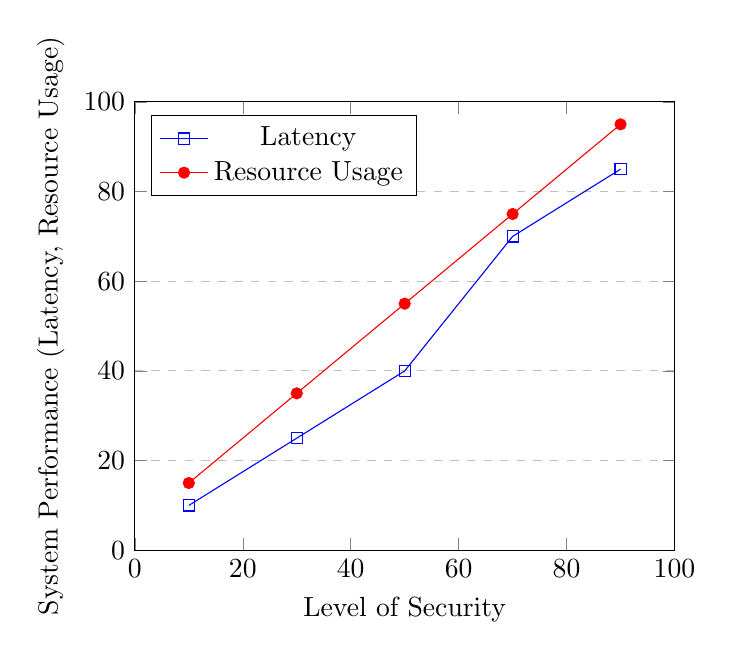
\begin{tikzpicture}
\begin{axis}[
    xlabel={Level of Security},
    ylabel={System Performance (Latency, Resource Usage)},
    xmin=0, xmax=100,
    ymin=0, ymax=100,
    legend pos=north west,
    ymajorgrids=true,
    grid style=dashed,
]
\addplot[
    color=blue,
    mark=square,
    ]
    coordinates {
    (10,10)(30,25)(50,40)(70,70)(90,85)
    };
\addlegendentry{Latency}

\addplot[
    color=red,
    mark=*,
    ]
    coordinates {
    (10,15)(30,35)(50,55)(70,75)(90,95)
    };
\addlegendentry{Resource Usage}

\end{axis}
\end{tikzpicture}
\caption{Impact of Security Measures on CPS Performance}
\label{fig:security_performance}
\end{figure}



\begin{table*}[h]
\centering
\caption{Overview of CPS Security Challenges, Impacts, and Mitigation Strategies}
\label{tab:cps_challenges}
\begin{tabular}{|p{4cm}|p{5cm}|p{5cm}|}
\hline
\textbf{Security Challenge} & \textbf{Impact} & \textbf{Mitigation Strategies} \\ \hline
Resource Constraints & Difficulty in applying strong security measures such as encryption due to limited computational capacity. & Use of lightweight cryptographic algorithms (e.g., ECC) and efficient anomaly detection techniques. \\ \hline
Legacy Systems & High vulnerability due to outdated protocols and hardware, leading to increased security risks. & Network segmentation, virtual patching, and incremental replacement of legacy components. \\ \hline
Cross-Domain Complexity & Integrated physical and cyber components create multiple attack surfaces, leading to increased risk of cyber-physical attacks. & Hybrid security approaches that monitor both physical and digital components simultaneously. \\ \hline
Scalability Issues & Difficulty in managing large numbers of interconnected devices, leading to cascading failure risks. & Hierarchical security management and segmentation to isolate failures and reduce overall risk. \\ \hline
Insider Threats & Harder to detect due to existing system privileges, posing risks of malicious or accidental attacks. & Multi-factor authentication (MFA), role-based access control (RBAC), and user behavior analytics (UBA). \\ \hline
Advanced Threats (e.g., Zero-day) & Vulnerabilities that are exploited before they can be patched, leading to potential system compromises. & Proactive threat modeling, rapid patch management, and machine learning-based detection systems. \\ \hline
\end{tabular}
\end{table*}



\usepackage{pgfplots}

\begin{figure}[h]
\centering
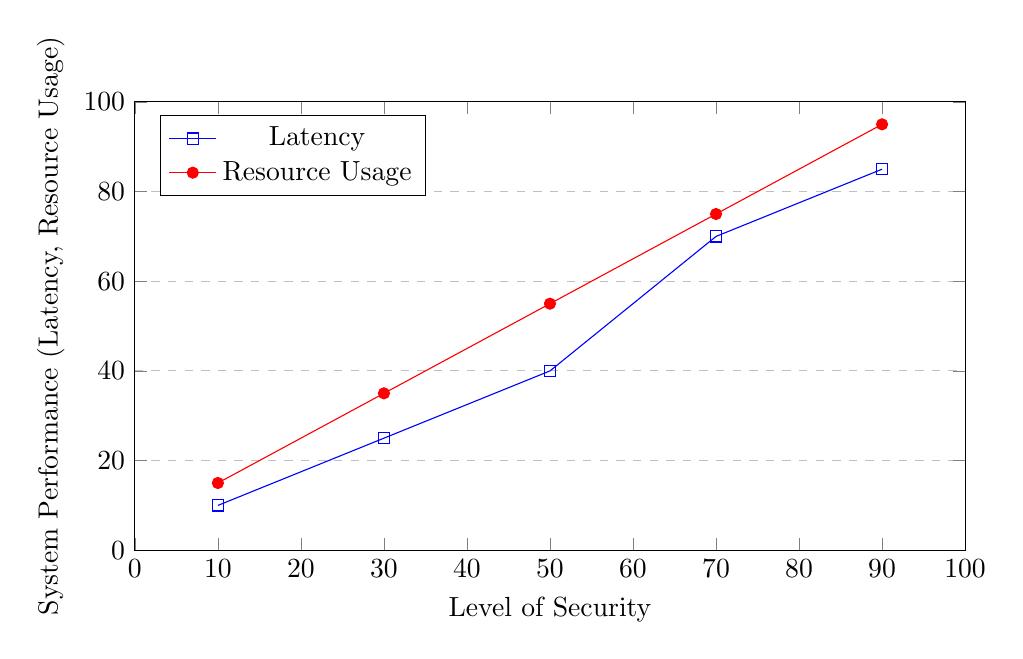
\begin{tikzpicture}
\begin{axis}[
    width=\linewidth,
    height=0.6\linewidth,
    xlabel={Level of Security},
    ylabel={System Performance (Latency, Resource Usage)},
    xmin=0, xmax=100,
    ymin=0, ymax=100,
    legend pos=north west,
    ymajorgrids=true,
    grid style=dashed,
]
% Plot for Latency
\addplot[
    color=blue,
    mark=square,
    ]
    coordinates {
    (10,10)(30,25)(50,40)(70,70)(90,85)
    };
\addlegendentry{Latency}

% Plot for Resource Usage
\addplot[
    color=red,
    mark=*,
    ]
    coordinates {
    (10,15)(30,35)(50,55)(70,75)(90,95)
    };
\addlegendentry{Resource Usage}

\end{axis}
\end{tikzpicture}
\caption{Impact of Security Measures on CPS Performance}
\label{fig:security_performance}
\end{figure}




\usetikzlibrary{shapes.geometric, arrows}

\tikzstyle{startstop} = [rectangle, rounded corners, minimum width=3cm, minimum height=1cm,text centered, draw=black, fill=red!30]
\tikzstyle{process} = [rectangle, minimum width=3cm, minimum height=1cm, text centered, draw=black, fill=orange!30]
\tikzstyle{decision} = [diamond, minimum width=3cm, minimum height=1cm, text centered, draw=black, fill=green!30]
\tikzstyle{arrow} = [thick,->,>=stealth]

\begin{figure*}[h]
\centering
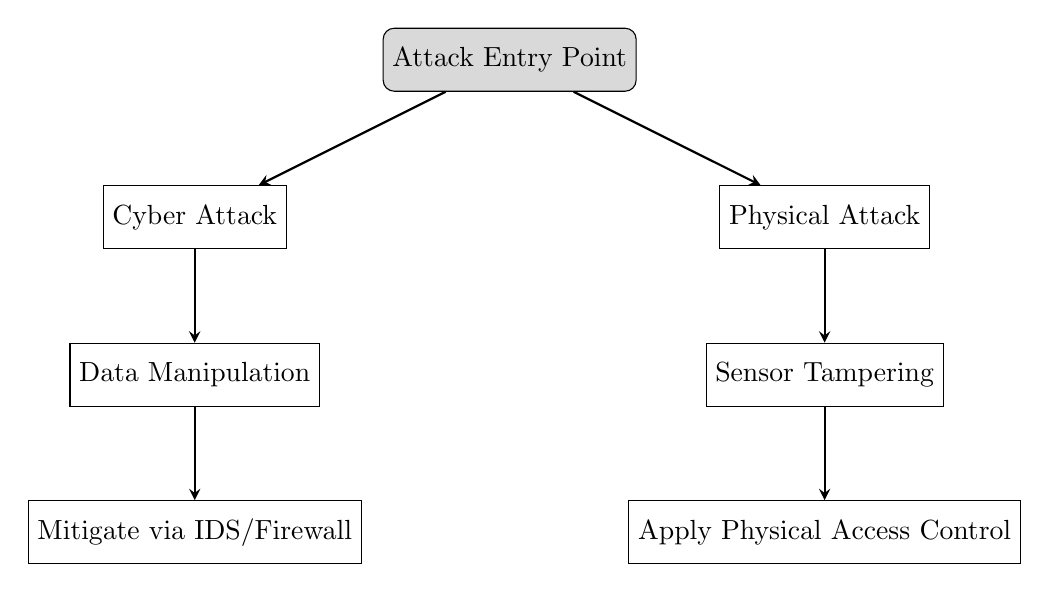
\begin{tikzpicture}[node distance=2cm]

% Nodes
\node (start) [startstop] {Attack Entry Point};
\node (cyber) [process, below of=start, xshift=-4cm] {Cyber Attack};
\node (physical) [process, below of=start, xshift=4cm] {Physical Attack};
\node (databreach) [process, below of=cyber] {Data Manipulation};
\node (tampering) [process, below of=physical] {Sensor Tampering};
\node (response1) [process, below of=databreach] {Mitigate via IDS/Firewall};
\node (response2) [process, below of=tampering] {Apply Physical Access Control};

% Arrows
\draw [arrow] (start) -- (cyber);
\draw [arrow] (start) -- (physical);
\draw [arrow] (cyber) -- (databreach);
\draw [arrow] (physical) -- (tampering);
\draw [arrow] (databreach) -- (response1);
\draw [arrow] (tampering) -- (response2);

\end{tikzpicture}
\caption{Attack Vectors and Response Pathways in CPS}
\label{fig:attack_pathways}
\end{figure*}




\usetikzlibrary{shapes, arrows, positioning}

\begin{figure*}[h]
\centering
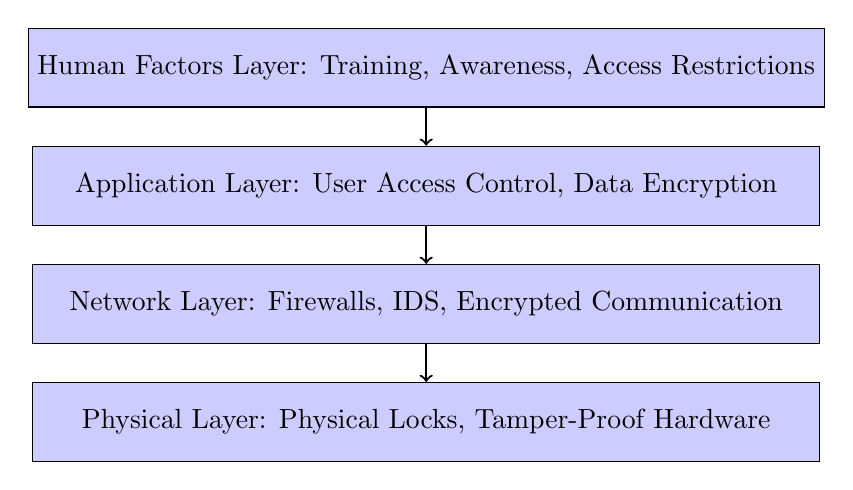
\begin{tikzpicture}[
    layer/.style={rectangle, draw=black, fill=blue!20, text centered, minimum width=10cm, minimum height=1cm},
    yscale=1.5
]

% Layers
\node[layer] (human) at (0,4) {Human Factors Layer: Training, Awareness, Access Restrictions};
\node[layer] (app) at (0,3) {Application Layer: User Access Control, Data Encryption};
\node[layer] (network) at (0,2) {Network Layer: Firewalls, IDS, Encrypted Communication};
\node[layer] (physical) at (0,1) {Physical Layer: Physical Locks, Tamper-Proof Hardware};

% Arrows
\draw[->, thick] (human.south) -- (app.north);
\draw[->, thick] (app.south) -- (network.north);
\draw[->, thick] (network.south) -- (physical.north);

\end{tikzpicture}
\caption{Security Layers in CPS Architecture}
\label{fig:security_layers}
\end{figure*}
\end{comment}

\section{CPS Security Challenges}\label{sec:challenges}
\begin{figure*}
\centering
\includegraphics[width=1\textwidth]{images/Schema.png}
\caption{Overview of CPS Security Challenges and Their Classifications}
\label{fig:overview-cps-challenges}
\end{figure*}


CPS face a wide range of security challenges due to their combination of digital and physical components. These systems, which are used in areas like healthcare, transportation, and critical infrastructure, must handle threats from both cyber and physical domains. The complexity of these systems makes them difficult to protect. To better understand these security issues, we can group them into four themes: system-level vulnerabilities, threats and attack types, security measures and responses, and external factors such as regulations, privacy concerns, and the human element \cite{166,167,168,169,170,171,172,173,174,175,176,177,178,179,180,181,182,183,184,185,186,187}. This section provides an integrated analysis of these challenges and explores possible solutions.

\subsection{System-Level Vulnerabilities and Constraints}

CPS face significant system-level vulnerabilities that stem from the resource limitations of their components, the cross-domain complexity of their architecture, and the continued use of legacy systems. Devices in CPS environments, such as sensors and actuators, often have constrained computational power, memory, and energy resources, making it difficult to implement standard security mechanisms like encryption and intrusion detection \cite{30,34,36}. These constraints are further compounded by the need for CPS to operate continuously without downtime, particularly in sectors where real-time operation is critical, such as healthcare and ICS\cite{31,36}. As a result, these systems cannot afford delays due to complex security updates or processes. To tackle these limitations, lightweight security solutions such as elliptic curve cryptography (ECC) and efficient anomaly detection techniques are increasingly adopted to balance the need for security with performance demands \cite{30,34}.

The cross-domain nature of CPS adds another layer of complexity to their security. Unlike traditional IT systems, CPS integrate both physical components such as machines, robots, and sensors with cyber elements, including networks and software \cite{209}. This tight coupling of the physical and cyber domains creates vulnerabilities that can be exploited by attackers in multiple ways \cite{31,34}. Attacks on CPS can target either the digital or the physical components; for instance, cyberattacks can manipulate sensor readings, while physical attacks can directly affect actuators or other hardware. Such attacks can lead to not only data breaches but also physical damage or significant threats to human safety \cite{30,34,40}.

Legacy systems pose additional challenges. Many CPS environments, particularly in critical infrastructure like power generation and healthcare, rely on legacy hardware and outdated protocols that were not designed with modern cybersecurity threats in mind \cite{40,42}. Updating or replacing these systems is often cost-prohibitive and operationally risky, leading to continued reliance on technology that lacks essential security capabilities. To mitigate the risks associated with these legacy systems, practices such as network segmentation and virtual patching are often used to create temporary security barriers \cite{40,42}.

The interconnectedness and scale of CPS also lead to challenges related to scalability and cascading effects. In large scale CPS networks such as smart cities or extensive industrial operations thousands of devices are interconnected, increasing the attack surface. If a single vulnerable component is compromised, it can trigger cascading failures that affect the entire system \cite{36,38}. For instance, a compromised sensor in a power grid could lead to widespread blackouts, as was observed in the 2003 Northeast blackout, where a failure in a single monitoring tool had far-reaching consequences \cite{37,41}. Hierarchical security management, where local control points are established to manage smaller segments of the network, is one approach that can help mitigate these risks by isolating failures and reducing overall system vulnerability \cite{37,41}.

\subsection{Threats and Attack Vectors}

CPS are exposed to a broad spectrum of threats, from traditional cyberattacks to physical sabotage, due to the diverse ways in which these systems operate and interact. One of the critical security challenges lies in the range and diversity of potential attack vectors. Digital attacks, such as malware, denial of service (DoS) attacks, and advanced persistent threats (APTs), can manipulate data or disrupt system operations \cite{30,34,40,201}. Meanwhile, physical threats such as tampering with sensors or other hardware can compromise the integrity of the physical components of the system \cite{30,34}. This dual nature of threats makes CPS security inherently more complex compared to traditional IT systems.

\begin{comment}
\begin{figure}[h]
\centering
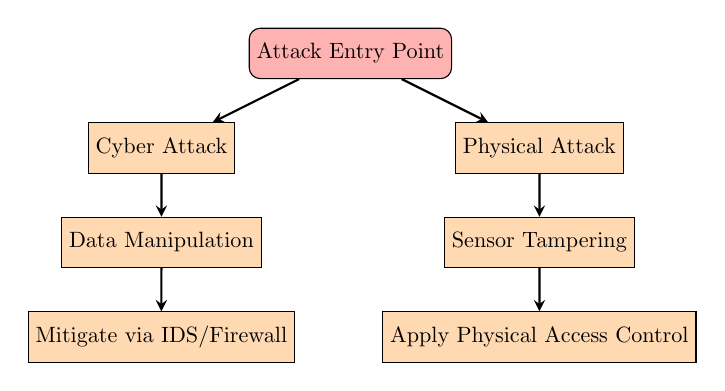
\begin{tikzpicture}[node distance=1.5cm, scale=0.8, every node/.style={transform shape}]
\tikzstyle{startstop} = [rectangle, rounded corners, minimum width=2.2cm, minimum height=0.8cm, text centered, draw=black, fill=red!30]
\tikzstyle{process} = [rectangle, minimum width=2.2cm, minimum height=0.8cm, text centered, draw=black, fill=orange!30]
\tikzstyle{arrow} = [thick,->,>=stealth]

% Nodes
\node (start) [startstop] {Attack Entry Point};
\node (cyber) [process, below of=start, xshift=-3cm] {Cyber Attack};
\node (physical) [process, below of=start, xshift=3cm] {Physical Attack};
\node (databreach) [process, below of=cyber] {Data Manipulation};
\node (tampering) [process, below of=physical] {Sensor Tampering};
\node (response1) [process, below of=databreach] {Mitigate via IDS/Firewall};
\node (response2) [process, below of=tampering] {Apply Physical Access Control};

% Arrows
\draw [arrow] (start) -- (cyber);
\draw [arrow] (start) -- (physical);
\draw [arrow] (cyber) -- (databreach);
\draw [arrow] (physical) -- (tampering);
\draw [arrow] (databreach) -- (response1);
\draw [arrow] (tampering) -- (response2);

\end{tikzpicture}
\caption{Attack Vectors and Response Pathways in CPS}
\label{fig:attack_pathways}
\end{figure}
\end{comment}


\begin{figure}[h]
\centering
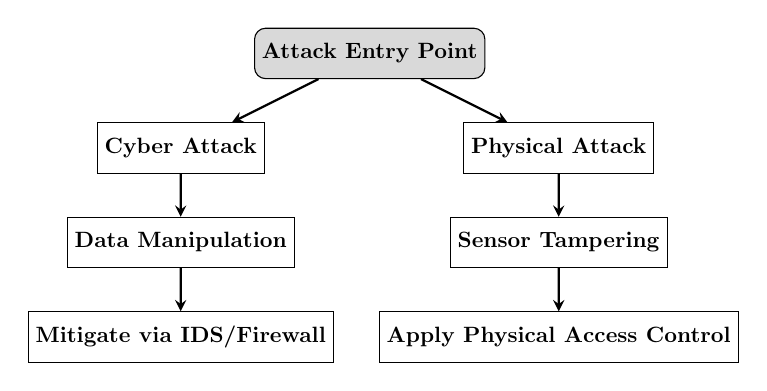
\begin{tikzpicture}[node distance=1.5cm, scale=0.8, every node/.style={transform shape}]
\tikzstyle{startstop} = [rectangle, rounded corners, minimum width=2.2cm, minimum height=0.8cm, text centered, draw=black, fill=gray!30]
\tikzstyle{process} = [rectangle, minimum width=2.2cm, minimum height=0.8cm, text centered, draw=black, fill=white]
\tikzstyle{arrow} = [thick,->,>=stealth, draw=black]

% Nodes
\node (start) [startstop] {\textbf{Attack Entry Point}};
\node (cyber) [process, below of=start, xshift=-3cm] {\textbf{Cyber Attack}};
\node (physical) [process, below of=start, xshift=3cm] {\textbf{Physical Attack}};
\node (databreach) [process, below of=cyber] {\textbf{Data Manipulation}};
\node (tampering) [process, below of=physical] {\textbf{Sensor Tampering}};
\node (response1) [process, below of=databreach] {\textbf{Mitigate via IDS/Firewall}};
\node (response2) [process, below of=tampering] {\textbf{Apply Physical Access Control}};

% Arrows
\draw [arrow] (start) -- (cyber);
\draw [arrow] (start) -- (physical);
\draw [arrow] (cyber) -- (databreach);
\draw [arrow] (physical) -- (tampering);
\draw [arrow] (databreach) -- (response1);
\draw [arrow] (tampering) -- (response2);

\end{tikzpicture}
\caption{The figure depicts typical attack entry points and the corresponding mitigation strategies in CPS, showcasing both digital and physical threat vectors.}
\label{fig:attack_pathways}
\end{figure}





Advanced threats, such as zero-day vulnerabilities, present a particularly serious risk to CPS because these vulnerabilities are often unknown to developers and security professionals \cite{203}, allowing attackers to exploit them before they are patched \cite{34,36,37}. Moreover, attackers are increasingly leveraging AI to identify vulnerabilities or automate coordinated attacks, further complicating defense mechanisms. Such attacks are difficult to detect because they may bypass conventional security measures, leading to potentially catastrophic outcomes, especially in critical systems like autonomous vehicles or industrial automation \cite{34,36}.

Insider threats add an additional dimension to the risk landscape of CPS. Insiders, such as employees or contractors, already have legitimate access to the system, making their actions difficult to detect and mitigate \cite{35,39}. These threats may be malicious or unintentional; for instance, a well-meaning employee could inadvertently misconfigure a device, introducing vulnerabilities. Mitigating these threats requires implementing robust access controls, such as multi-factor authentication (MFA) and role-based access control (RBAC), and using user behavior analytics (UBA) to detect abnormal activities that might indicate an insider threat \cite{35,39}.

Figure \ref{fig:attack_pathways} illustrates the typical attack entry points in CPS, categorizing them into cyber attacks and physical attacks, along with corresponding mitigation strategies that address digital threats through IDS/Firewalls and physical threats via access control measures.
\subsection{Security Measures and Responses}

Effective CPS security demands a comprehensive approach that integrates multiple protective measures across both the cyber and physical domains. Traditional security tools, such as firewalls and network-based intrusion detection systems, are insufficient on their own, as CPS require defenses that span both digital data flows and physical operations \cite{30,33}. An emerging approach to enhance CPS security involves using hybrid intrusion detection systems that combine machine learning-based anomaly detection with traditional signature-based techniques. These hybrid systems are particularly effective at identifying both known and emerging threats, providing a more holistic defense against complex attack scenarios \cite{30,33}.

Another essential aspect of securing CPS is ensuring resilience in the face of attacks. CPS must be capable of detecting and isolating security breaches swiftly while continuing to operate without causing harm \cite{33,41}. For example, in a smart grid, if one segment is compromised, other parts of the grid must maintain functionality to prevent a large-scale blackout. Resilience can be built into CPS through redundancy, failover mechanisms, and segmentation, allowing the system to withstand localized attacks without experiencing total failure \cite{33,41}.

\begin{figure}[h]
\centering
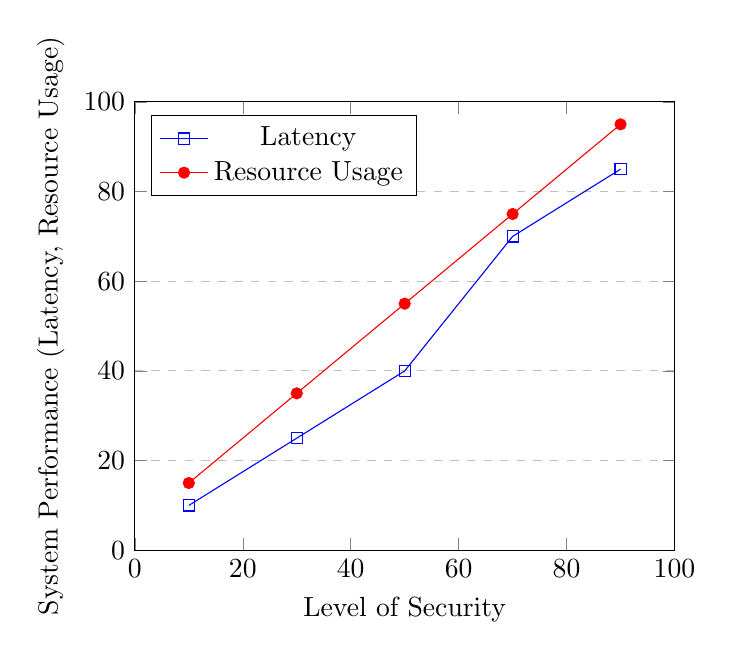
\begin{tikzpicture}
\begin{axis}[
    xlabel={Level of Security},
    ylabel={System Performance (Latency, Resource Usage)},
    xmin=0, xmax=100,
    ymin=0, ymax=100,
    legend pos=north west,
    ymajorgrids=true,
    grid style=dashed,
]
\addplot[
    color=blue,
    mark=square,
    ]
    coordinates {
    (10,10)(30,25)(50,40)(70,70)(90,85)
    };
\addlegendentry{Latency}

\addplot[
    color=red,
    mark=*,
    ]
    coordinates {
    (10,15)(30,35)(50,55)(70,75)(90,95)
    };
\addlegendentry{Resource Usage}

\end{axis}
\end{tikzpicture}
\caption{Impact of Security Measures on CPS Performance}
\label{fig:security_performance}
\end{figure}

The need for real-time responsiveness is another critical factor in CPS security. Implementing advanced security measures, such as encryption or multifactor authentication, can sometimes introduce latency, which can be unacceptable in systems requiring immediate response, such as healthcare devices or autonomous vehicles \cite{30,31,33}. Figure~\ref{fig:security_performance} illustrates how increasing levels of security impact key performance metrics like latency and resource usage, highlighting the importance of balancing security with operational efficiency. Recent advances, like homomorphic encryption enabling operations on encrypted data without decryption and edge computing processing data closer to the source can offer solutions that enhance security while maintaining the necessary performance levels \cite{30,31,33}.

\subsection{Regulatory, Privacy, and Human Factors}

Beyond the technical challenges, CPS security is also influenced by regulatory, privacy, and human factors. The regulatory landscape for CPS is fragmented, with some sectors, such as electric power, adopting rigorous standards like the North American Electric Reliability Corporation (NERC) guidelines, while others lack comprehensive regulations \cite{30,32,42}. This inconsistency creates gaps in the security posture of different CPS sectors. Developing a unified international regulatory framework drawing on models like ISO/IEC 27001 but tailored for CPS environments could help establish a standardized level of security across industries.
\begin{comment}
    
\begin{figure}[h]
\centering
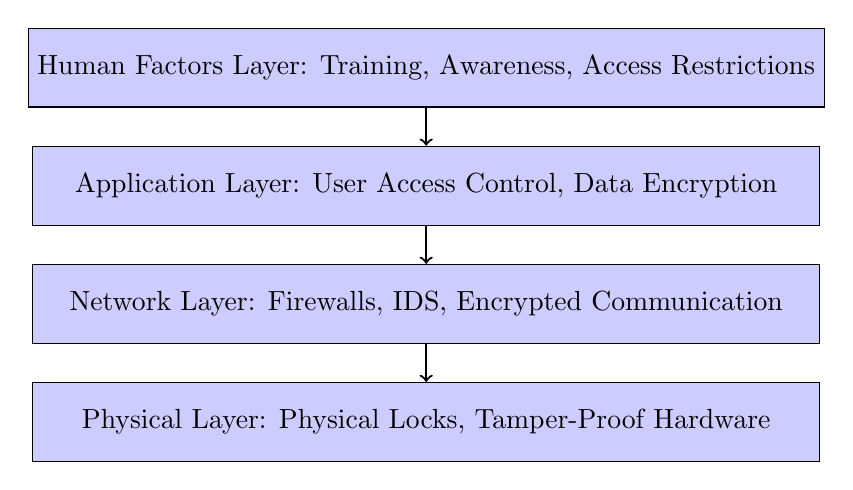
\begin{tikzpicture}[
    layer/.style={rectangle, draw=black, fill=blue!20, text centered, minimum width=10cm, minimum height=1cm},
    yscale=1.5
]

% Layers
\node[layer] (human) at (0,4) {Human Factors Layer: Training, Awareness, Access Restrictions};
\node[layer] (app) at (0,3) {Application Layer: User Access Control, Data Encryption};
\node[layer] (network) at (0,2) {Network Layer: Firewalls, IDS, Encrypted Communication};
\node[layer] (physical) at (0,1) {Physical Layer: Physical Locks, Tamper-Proof Hardware};

% Arrows
\draw[->, thick] (human.south) -- (app.north);
\draw[->, thick] (app.south) -- (network.north);
\draw[->, thick] (network.south) -- (physical.north);

\end{tikzpicture}
\caption{Security Layers in CPS Architecture}
\label{fig:security_layers}
\end{figure}
\end{comment}

\begin{comment}
\begin{table}[h]
\centering
\caption{Some Impact and Mitigation Strategies of CPS Security Challenges}
\label{tab:cps_challenges}
\begin{tabular}{|p{1.5cm}|p{3cm}|p{3cm}|}
\hline
\textbf{Security Challenge} & \textbf{Impact} & \textbf{Mitigation Strategies} \\ \midrule
Resource Constraints & Difficulty in applying strong security measures such as encryption due to limited computational capacity. & Use of lightweight cryptographic algorithms (e.g., ECC) and efficient anomaly detection techniques \cite{30,34,36}. \\ \midrule
Legacy Systems & High vulnerability due to outdated protocols and hardware, leading to increased security risks. & Network segmentation, virtual patching, and incremental replacement of legacy components \cite{40,42}. \\ \midrule
Cross-Domain Complexity & Integrated physical and cyber components create multiple attack surfaces, leading to increased risk of cyber-physical attacks. & Hybrid security approaches that monitor both physical and digital components simultaneously \cite{31,34}. \\ \midrule
Scalability Issues & Difficulty in managing large numbers of interconnected devices, leading to cascading failure risks. & Hierarchical security management and segmentation to isolate failures and reduce overall risk \cite{36,38}. \\ \midrule
Insider Threats & Harder to detect due to existing system privileges, posing risks of malicious or accidental attacks. & Multi-factor authentication (MFA), role-based access control (RBAC), and user behavior analytics (UBA) \cite{35,39}. \\ \midrule
Advanced Threats (e.g., Zero-day) & Vulnerabilities that are exploited before they can be patched, leading to potential system compromises. & Proactive threat modeling, rapid patch management, and machine learning-based detection systems \cite{34,36,37}. \\ \midrule
\end{tabular}
\end{table}
\end{comment}



\begin{table*}[h]
\centering
\caption{Some Impact and Mitigation Strategies of CPS Security Challenges}
\label{tab:cps_challenges}
\renewcommand{\arraystretch}{1.3}
\begin{tabularx}{\textwidth}{@{}p{2.5cm}X X@{}}
\toprule
\textbf{Security Challenge} & \textbf{Impact} & \textbf{Mitigation Strategies} \\
\midrule
Resource Constraints & Difficulty in applying strong security measures such as encryption due to limited computational capacity. & Use of lightweight cryptographic algorithms (e.g., ECC) and efficient anomaly detection techniques \cite{30,34,36} \\
\addlinespace
\rowcolor[HTML]{EFEFEF}
Legacy Systems & High vulnerability due to outdated protocols and hardware, leading to increased security risks. & Network segmentation, virtual patching, and incremental replacement of legacy components \cite{40,42} \\
\addlinespace

Cross-Domain Complexity & Integrated physical and cyber components create multiple attack surfaces, leading to increased risk of cyber-physical attacks. & Hybrid security approaches that monitor both physical and digital components simultaneously \cite{31,34} \\
\addlinespace
\rowcolor[HTML]{EFEFEF}
Scalability Issues & Difficulty in managing large numbers of interconnected devices, leading to cascading failure risks. & Hierarchical security management and segmentation to isolate failures and reduce overall risk \cite{36,38} \\
\addlinespace
Insider Threats & Harder to detect due to existing system privileges, posing risks of malicious or accidental attacks. & Multi-factor authentication (MFA), role-based access control (RBAC), and user behavior analytics (UBA) \cite{35,39} \\
\addlinespace
\rowcolor[HTML]{EFEFEF}
Advanced Threats& Vulnerabilities that are exploited before they can be patched, leading to potential system compromises. & Proactive threat modeling, rapid patch management, and machine learning-based detection systems \cite{34,36,37} \\
\bottomrule
\end{tabularx}
\end{table*}

\begin{comment}
\begin{table*}[htbp]
\centering
\caption{Some Impact and Mitigation Strategies of CPS Security Challenges}
\label{tab:cps_challenges}
\renewcommand{\arraystretch}{1.3}  % Increase vertical spacing
\begin{tabular}{|p{2.5cm}|p{5cm}|p{5cm}|}
\hline
\rowcolor{gray!10}  % Add light gray background to header
\textbf{Security Challenge} & \textbf{Impact} & \textbf{Mitigation Strategies} \\
\hline
\textbf{Resource Constraints} & 
Difficulty in applying strong security measures such as encryption due to limited computational capacity. & 
Use of lightweight cryptographic algorithms (e.g., ECC) and efficient anomaly detection techniques \cite{30,34,36}. \\
\hline
\rowcolor{gray!5}  % Alternate row color
\textbf{Legacy Systems} & 
High vulnerability due to outdated protocols and hardware, leading to increased security risks. & 
Network segmentation, virtual patching, and incremental replacement of legacy components \cite{40,42}. \\
\hline
\textbf{Cross-Domain Complexity} & 
Integrated physical and cyber components create multiple attack surfaces, leading to increased risk of cyber-physical attacks. & 
Hybrid security approaches that monitor both physical and digital components simultaneously \cite{31,34}. \\
\hline
\rowcolor{gray!5}  % Alternate row color
\textbf{Scalability Issues} & 
Difficulty in managing large numbers of interconnected devices, leading to cascading failure risks. & 
Hierarchical security management and segmentation to isolate failures and reduce overall risk \cite{36,38}. \\
\hline
\textbf{Insider Threats} & 
Harder to detect due to existing system privileges, posing risks of malicious or accidental attacks. & 
Multi-factor authentication (MFA), role-based access control (RBAC), and user behavior analytics (UBA) \cite{35,39}. \\
\hline
\rowcolor{gray!5}  % Alternate row color
\textbf{Advanced Threats} \newline (e.g., Zero-day) & 
Vulnerabilities that are exploited before they can be patched, leading to potential system compromises. & 
Proactive threat modeling, rapid patch management, and machine learning-based detection systems \cite{34,36,37}. \\
\hline
\end{tabular}
\end{table*}

    
\end{comment}


Data integrity and privacy are also critical concerns. CPS often collect significant amounts of sensitive data, especially in applications like healthcare and smart cities \cite{31,36,38}. Ensuring this data remains secure from unauthorized access is crucial to preventing attackers from manipulating system behavior. At the same time, privacy must be maintained, particularly where personal user data is involved. Designers need to strike a delicate balance between functionality and privacy by integrating privacy-by-design principles into CPS development \cite{31,36}.

Human factors, particularly the lack of specialized security training among CPS operators and engineers, pose additional challenges. Many employees responsible for managing CPS do not have sufficient training to recognize or mitigate security threats effectively \cite{39,43}. Programs like the NIST Cybersecurity Workforce Framework can provide organizations with a structure to identify skill gaps and improve security awareness through training and education. Enhancing workforce competence is crucial for preventing unintentional security breaches and ensuring that CPS are properly managed and protected \cite{39,43}.

Table \ref{tab:cps_challenges} provides some examples of CPS security challenges, illustrating their impacts and mitigation strategies, such as the use of lightweight cryptographic algorithms for addressing resource constraints and hybrid security approaches for managing cross-domain complexity.

The security of CPS is shaped by a multitude of interrelated challenges that include technical limitations, complex attack vectors, the need for specialized security measures, and broader regulatory and human factors. Addressing these challenges requires an integrated approach that combines technological innovation, strategic policy-making, and investment in human capital \cite{188,189,190,191,192,193}. Such a comprehensive strategy will be essential to secure CPS as they continue to expand and play an increasingly critical role in our interconnected world. Diagram \ref{fig:overview-cps-challenges} provides a structured overview of the primary security challenges in CPS, categorized into system vulnerabilities, attack vectors, mitigation measures, and external factors.
